\documentclass[10pt,a4paper]{article}
\usepackage[utf8]{inputenc}
\usepackage[T1]{fontenc}
\usepackage[polish]{babel}
\usepackage{amsmath}
\usepackage{amsfonts}
\usepackage{amssymb}
\usepackage{graphicx}
\author{Jakub Jaśków}
\title{Obliczenia Naukowe - Lista nr 2}
\begin{document}
\maketitle
\section{Zad}
\subsection*{Opis}
Powtórzyć zadanie 5 z listy 1. Usunąć ostatnią 9 z $x_4$ i ostatnią 7 z $x_5$. Porównać i objaśnić wyniki.
\subsection*{Rozwiązanie}
Modyfikujemy kod z zadania 5 listy 1 tak aby wartości odpowiadały tym z polecenia.
\subsection*{Wyniki}
\begin{center}
\begin{tabular}{|l|l|l|l|}
\hline
\textbf{Float32} & \textbf{Function} & \textbf{New} & \textbf{Old} \\
\hline
& forwards() & -0.4999443 & -0.4999443 \\
& backwards() & -0.4543457 & -0.4543457 \\
& maxToMax() & -0.5 & -0.5 \\
& revmaxToMax() & -0.5 & -0.5 \\
\hline
\textbf{Float64} & \textbf{Function} & \textbf{New} & \textbf{Old} \\
\hline
& forwards() & -0.004296342739891585 & 1.0251881368296672e-10 \\
& backwards() & -0.004296342998713953 & -1.5643308870494366e-10 \\
& maxToMax() & -0.004296342842280865 & 0.0 \\
& revmaxToMax() & -0.004296342842280865 & 0.0 \\
\hline
\end{tabular}
\end{center}

Jak widać wyniki algorytmów dla typu \textbf{Float32} są takie same. Nie jest to szokujące, ponieważ zmiany w danych zostały dokonane na końcach precyzji \textbf{Float32}.

Wyniki dla \textbf{Float64} różnią się jednak znacząco. Porównujące je do prawidłowej nowej wartości $sum(x',y) = -0.004296343192495245$ widzimy, że nowe wyniki nie tak bardzo różnią się od wartości prawidłowych. Różnica jest rzędu $10^-10$
\subsection*{Wnioski}
Zauważyć możemy, że o ile błąd bezwzględny dla obu danych wejściowych mają podobny rząd wielkości to wartości iloczynu znacząco się zmieniła, w wyniku czego błąd względny drastycznie zmalał. Wartość realna iloczynu skalarnego znacznie się zmieniła.

Na skutek wyżej wymienionych obserwacji możemy wywnioskować, że to nie wina dopasowania naszych algorytmów, ale uwarunkowanie zadania sprawia, że niewielkie zmiany danych wejściowych w znaczny sposób wpływają na wyniki.
\section{Zad}
\subsection*{Opis}
Narysować wykres funkcji $f(x)=e^{x}ln(1+e^{-x})$ w co najmniej dwóch programach do wizualizacji. Policzyć granicę funkcji przy $lim_{x\rightarrow\infty}f(x)$. Porównać wykres funkcji z jej granicą i wyjaśnić zjawisko.
\subsection*{Rozwiązanie}
Do rozwiązania tego zadania użyjemy 4 różnych programów graficzny: \textbf{Wolfram Alpha}, \textbf{Symbolab}, \textbf{Julia}, \textbf{Desmos}.
Wartości przedstawione na wykresach porównamy z limitem funkcji $lim_{x\rightarrow\infty}(e^{x}ln(1+e^{-x})) = 1$.
\subsection*{Wyniki}
\begin{figure}[hbt!]
\caption{Desmos}
\centering
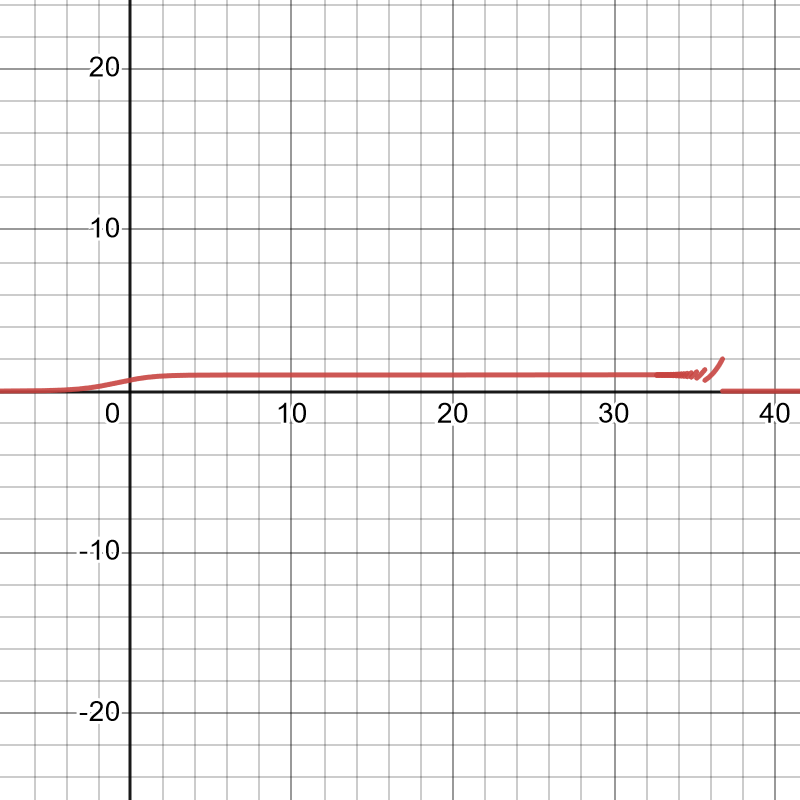
\includegraphics[scale=0.2]{D:/Repozytoria/Studies/sem5/ON/L2/plots/ex2/desmos.png}
\end{figure}
\begin{figure}[hbt!]
\caption{Wolfram Alpha - przybliżenie}
\centering
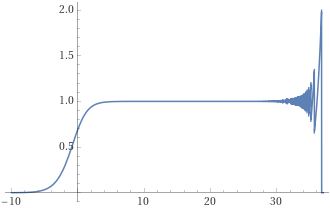
\includegraphics[scale=0.5]{D:/Repozytoria/Studies/sem5/ON/L2/plots/ex2/wolfram-alpha-closeup.png}
\end{figure}
\begin{figure}[hbt!]
\caption{Julia - przybliżenie}
\centering
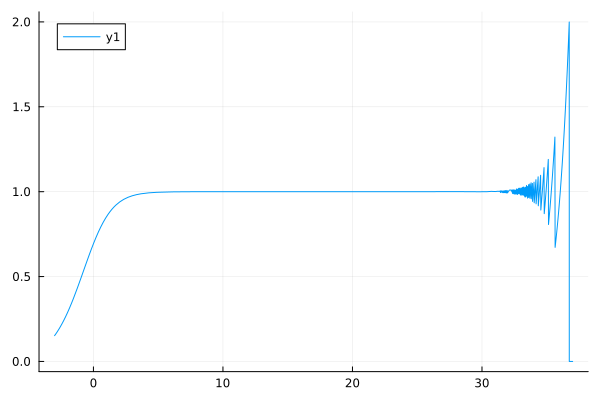
\includegraphics[scale=0.3]{D:/Repozytoria/Studies/sem5/ON/L2/plots/ex2/julia-closeup.png}
\end{figure}
\begin{figure}[hbt!]
\caption{Symbolab - przybliżenie}
\centering
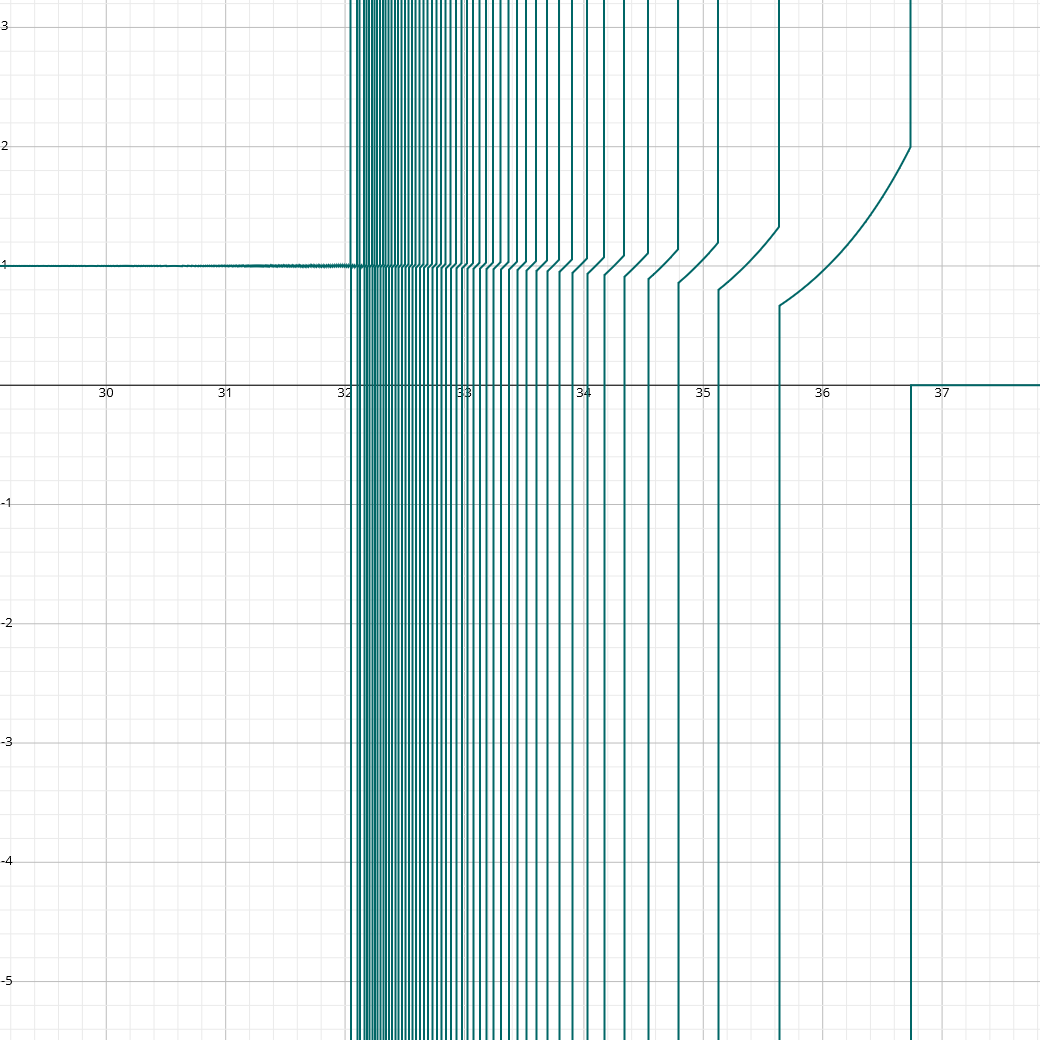
\includegraphics[scale=0.11]{D:/Repozytoria/Studies/sem5/ON/L2/plots/ex2/symbolab-closeup.png}
\end{figure}
Widać, że wykresy różnią się od prawdziwych wartości funkcji.
\subsection*{Wnioski}
Wartość granicy funkcji odczytana z wykresu znacząco różni się od tej wyliczonej ręcznie. Dzieje się tak ponieważ dla dużych $x$ wyrażenie w środku logarytmu $1+e^{-x} = 1+( \frac{1}{e^x})  \approx 1$, a $e^x*ln(1) = e^x*0=0$. Możemy zatem wnioskować, że zadanie to jest źle uwarunkowane, co potwierdzają aż 4 wykresy z odrębnych programów graficzno-matematycznych.
\section{Zad}
\subsection*{Opis}
\subsection*{Rozwiązanie}
\subsection*{Wyniki}
\subsection*{Wnioski}
\section{Zad}
\subsection*{Opis}
\subsection*{Rozwiązanie}
\subsection*{Wyniki}
\subsection*{Wnioski}
\section{Zad}
\subsection*{Opis}
\subsection*{Rozwiązanie}
\subsection*{Wyniki}
\subsection*{Wnioski}
\section{Zad}
\subsection*{Opis}
\subsection*{Rozwiązanie}
\subsection*{Wyniki}
\subsection*{Wnioski}
\section{Zad}
\subsection*{Opis}
\subsection*{Rozwiązanie}
\subsection*{Wyniki}
\subsection*{Wnioski}
\end{document}